Seguindo para os resutlados das arquiteturas com poucos parâmetros, a primeira destas a ser treinada e testada foi a MobileNet. Para esta arquitetura, considerando ambas as abordagens, foi realizada mais uma vez uma busca em \emph{grid} de modelos utilizando todos os hiperparâmetros especificados anteriormente, gerando um total de $72$ modelos diferentes.

Nesta arquitetura em particular, foi considerada a métrica de EER para a escolha dos melhores modelos e estes encontram-se presentes na Tabela \ref{tab:mobilenet}. Na Figura \ref{fig:treinamento-mobilenet} pode-se observar os gráficos com o comportamento da \emph{loss} e acurácia dos conjuntos de treino e validação durante a etapa de ajustamento dos modelos.

\begin{table}[h!]
\centering
\caption{Detalhamento dos melhores modelos obtidos com a arquitetura MobileNet para cada uma das abordagens consideradas neste trabalho.}
\label{tab:mobilenet}
\resizebox{\textwidth}{!}{\begin{tabular}{ccccccc}
\toprule
\textbf{Abordagem} & \textbf{Otimizador} & \textbf{\emph{Patience}}  & \textbf{Função de Ativação} & \textbf{Acurácia} & \textbf{F-Score} & \textbf{EER} \\
\midrule
Abordagem A & SGD & 15 & ReLU & $0.9606$ & $0.9318$ & $0.9304$ \\
Abordagem B & Adam & 15 & ReLU & $0.8856$ & $0.8658$ & $9.9475$\\
\bottomrule
\end{tabular}}
\end{table}

\begin{figure}[H]
\centering
\caption{Histórico de \emph{loss} e acurácia durante o treinamento dos melhores modelos obtidos com a arquitetura MobileNet.}
\label{fig:treinamento-mobilenet}
\subfloat[\emph{Loss} durante treinamento da melhor rede MobileNet para a abordagem A.\label{subfig:mobilenet-a-loss}]{%
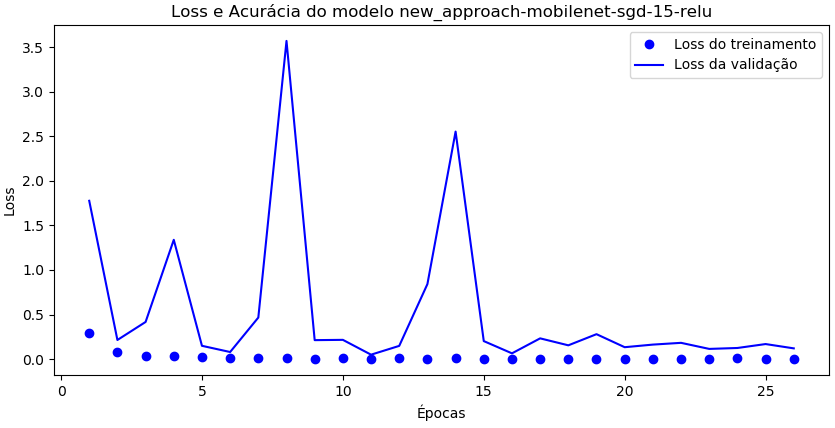
\includegraphics[width=0.47\textwidth]{imgs/mobilenet-a-loss}
}
\hfill
\subfloat[Acurácia durante treinamento da melhor rede MobileNet para a abordagem A.\label{subfig:mobilenet-a-acc}]{%
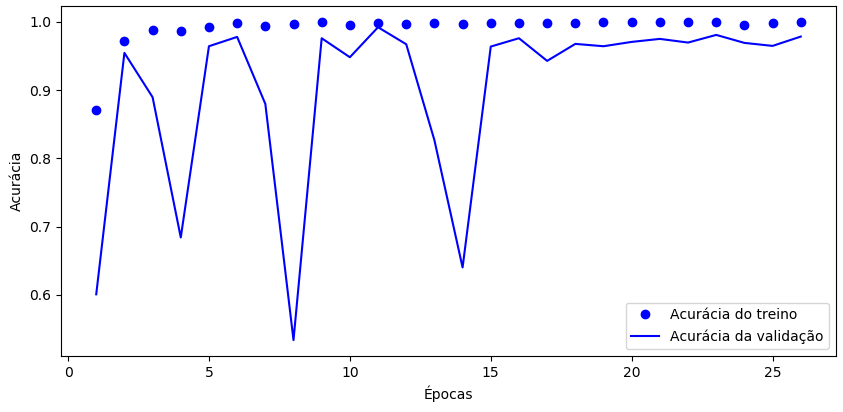
\includegraphics[width=0.47\textwidth]{imgs/mobilenet-a-acc}
}
\hfill
\subfloat[\emph{Loss} durante treinamento da melhor rede MobileNet para a abordagem B.\label{subfig:mobilenet-b-loss}]{%
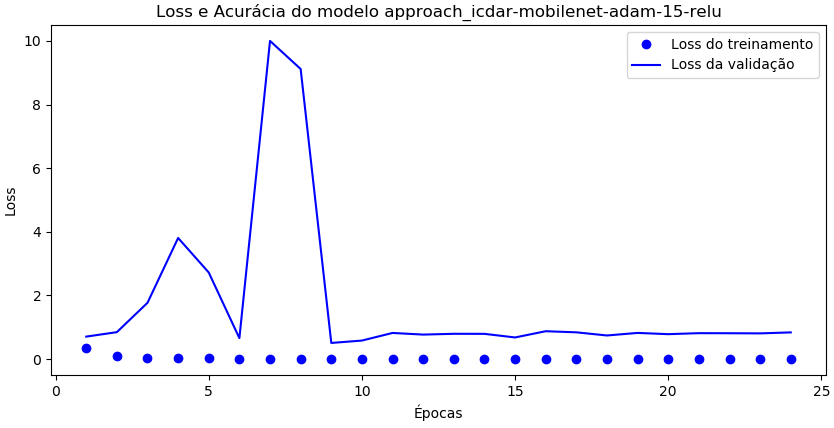
\includegraphics[width=0.47\textwidth]{imgs/mobilenet-b-loss}
}
\hfill
\subfloat[Acurácia durante treinamento da melhor rede MobileNet para a abordagem B.\label{subfig:mobilenet-b-acc}]{%
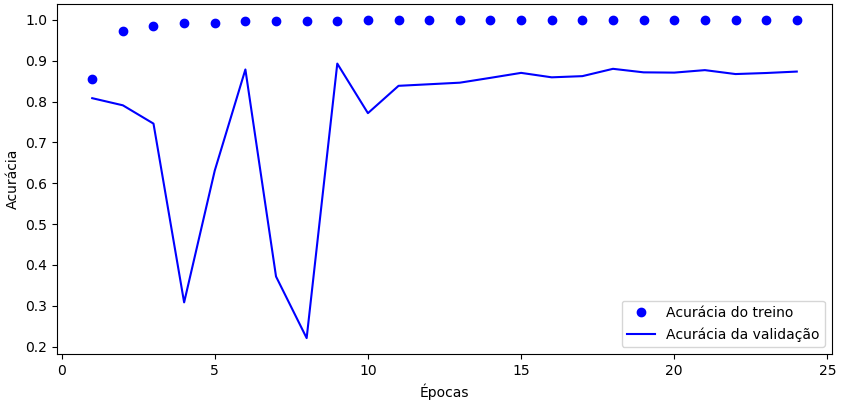
\includegraphics[width=0.47\textwidth]{imgs/mobilenet-b-acc}
}
\end{figure}

Dentre as CNNs observadas até o momento, a MobileNet foi a que obteve um melhor desempenho. Isso se deve, possivelmente, aos poucos padrões encontrados nas imagens de treinamento, por se tratar de imagens em escala de cinza, e à existência de poucos parâmetros treináveis para esta arquitetura. Essas duas características se fizeram essenciais para a descoberta de modelos superiores aos demais, quando analisando apenas a métrica de EER.

Na Figura \ref{fig:matrizes-mobilenet} pode-se visualizar as matrizes de confusão obtidas pelos melhores modelos. Percebe-se que, para abordagem A, apesar da diagonal principal densa, a quantidade de falsos negativos foi maior do que o encontrado nas arquiteturas anteriores para a mesma abordagem. Quanto à matriz encontrada para a abordagem B, podemos considerar as mesmas reflexões concebidas à matriz da arquitetura LeNet.

\begin{figure}[h]
	\centering
	\caption{Matrizes de confusão dos melhores modelos obtidos com a arquitetura MobileNet.}\label{fig:matrizes-mobilenet}
	\subfloat[Melhor MobileNet com a abordagem A\label{subfig:matriz-mobilenet-a}]{%
	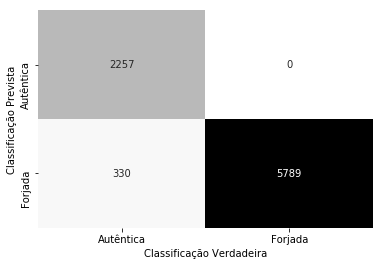
\includegraphics[width=0.47\textwidth]{imgs/matriz-mobilenet-a}
	}
	\hfill
	\subfloat[Melhor MobileNet com a abordagem B\label{subfig:matriz-mobilenet-b}]{%
	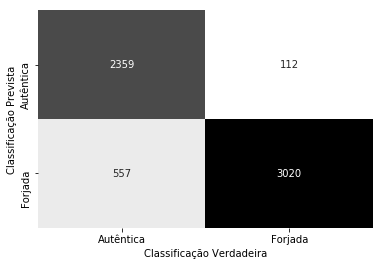
\includegraphics[width=0.47\textwidth]{imgs/matriz-mobilenet-b}
	}
\end{figure}